
\RequirePackage{fix-cm}
\documentclass{svjour3}     
\usepackage[francais]{babel}
\usepackage[utf8]{inputenc}
\usepackage[T1]{fontenc}
\usepackage{graphicx}
\usepackage{listings}
\smartqed  % flush right qed marks, e.g. at end of proof
%
\usepackage{tikz}
\usetikzlibrary{arrows,positioning,automata,shadows}
%
 \usepackage{mathptmx}      % use Times fonts if available on your TeX system
%
% insert here the call for the packages your document requires
\usepackage{latexsym}
% etc.
%
% please place your own definitions here and don't use \def but
% \newcommand{}{}
%
% Insert the name of "your journal" with
% \journalname{myjournal}
%
\begin{document}

\title{Compilation and diagnosis for discrete controller synthesis}
%\subtitle{Compilation et diagnostics de la synthèse de  contrôleurs discrets}

%\titlerunning{Compilation et diagnostics de la synthèse de  contrôleurs discrets}        % if too long for running head

\author{Seydou coulibaly  \\ \and \\
        Encadré par : Gwenaël Delaval.
}

\authorrunning{Short form of author list} % if too long for running head

\institute{Seydou coulibaly \at
              Saint martin d'heres, 38400, France \\
              \email{cseydou28@gmail.com}           %  \\
%             \emph{Present address:} of F. Author  %  if needed
           \and
           S. Author \at
              second address
}

\date{Juin 2016}
% The correct dates will be entered by the editor

\maketitle

\begin{abstract}
Cet article présente la compilation de la synthèse des contrôleurs discrets avec le Diagnostic de ce dernier. La synthèse de contrôleurs discrets est une méthode
de conception qui génère des contrôleurs pour le contrôle d'un système devant vérifié certaines propriétés. Les approches les plus souvent utilis\'ees 
pour sa conception sont la th\'eorie des automates, les r\'eseaux de pétri, la th\'eorie des jeux. Dans ce travail, le contrôleur est intégrée dans un langage
synchrone flots de données capable de réprésenter les spécifications d'un système sous forme d'automates à état fini. Ce langage inclue le mécanisme de contrat, 
necessaire pour la génération de contrôleurs. Tout au long de ce rapport, d\'ecoulera la présentation du langage Heptagon/BZR, les résultats possibles de sa 
compilation qui sont variés tels que les échecs de la synthèse de contrôleurs discrets et la réalisation d'un exemple assez concret. Le choix des exemples de syst\`emes \`a concevoir reste vastes mais cadr\'e au 
tour des syst\`emes pouvant \^etre mod\'eliser par des langages synchrones comme par exemple les syst\`emes automatiques, les syst\`emes industrielles, 
les automates programmables. \newline Heptagon/BZR a \'egalement la particularit\'e d'\^etre r\'eactif assurant une leg\`ere mod\'elisation de telle syst\`emes qui sont
g\'eneralement critique, deterministe et surtout incluant la notion de parrall\'elisme .
C'est un programme qui décrit sous forme d'automates les comportements d'un système en premettant la mod\'elisation de ses \'etats, 
ses transitions, ses sorties ainsi que leurs actions. 
\keywords{langage synchrone \and compilation \and syntheses de controleurs discretes \and BZR \and Heptagon \and Reax \and syst\`eme reactif \and contrats \and CTRL-A}
% \PACS{PACS code1 \and PACS code2 \and more}
% \subclass{MSC code1 \and MSC code2 \and more}
\end{abstract}

\section{Introduction}
\label{intro}
On s'interesse à la compilation et au Diagnostic de la synthèse des contrôleurs discrets, une méthode de conception et de validation permettant de contrôler un système 
au tour d'un environement ou d'une propriéte. Des outils de synthèse de contrôleurs existent déja dont REAX et SIGALI \cite{wodes-Reax} \cite{marchand00c}. Il est intégrable dans un 
langage de programmation, spécifiquement un langage synchrone et tout au long de ce document, on utilisera le langage Heptagon/BZR qu'en est un exemple
pour nos analyses et interprétations.


Heptagon/BZR est un langage synchrone flots de données utilisé pour programmer des systèmes réactifs. Il décrit sous forme d'automate les comportements
possible d'un système. Sa compilation produit des résultats assez variés, des problèmes de syntaxe, des échecs de la synthèse de contrôleurs discrets
et des cas où la synthèse reussie bien à générer une logique de contrôle mais que le système obtenu n'arrive pas à repondre à la spécification initiale du système 
au dela des contraintes. Ce document décrit ainsi les éventuels résultats possible de la compilation de la synthèse de contrôleurs discrets.

\subsection{La synthèse de contrôleurs discrets}
La synthèse de contrôleurs discrets consiste à reduire le comportement d'un système P par le biais d'un superviseur ou contrôleur C de manière 
à ce que le système ainsi contrôlé soit correct vis à vis d'un ensemble de propriétes D (ou d'objectifs de contrôle) que le système initial ne verifiat pas. 
Plus spécifiquement, c'est une méthode qui genère un contrôleur (une logique de contrôle) sur un système de sorte que le comportement de ce dernier 
soit conforme à celui désiré \cite{ref8}. La synthèse de contrôleurs discrets est appliquée sur des systèmes réprésentés par un ensemble de comportements 
comme sous la forme d'automates finis, de réseaux de pétri ou sous la forme de systèmes de transition symboliques, etc. De tels systèmes sont constitués de sorties
et d'entrées, généralement classées dans deux catégories, les entrées contrôlables et les les entrées incontrôlables. La synthèse de contrôleurs n'a d'habilité 
d'agir que sur les entrées contrôlables et n'a aucun effet sur les entrées incontrôlables qui proviennent de l'environement (capteurs, des actions de l'utilisateur, 
évènements extérieurs au système) \cite{drm13}.  Peu connue des programmeurs, la synthèse de contrôleurs est apparue dans les ann\'ees 1980. C'est un domaine
de recherche à part entière et reste l'une des m\'ethodes de conception et de validation les plus difficiles à concevoir avec beaucoup de notions au tour.
\begin{figure}[!h]
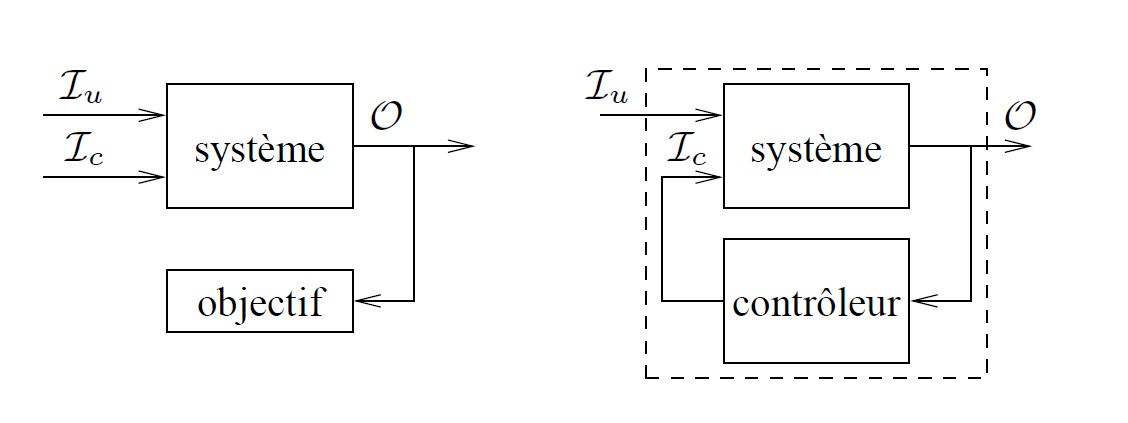
\includegraphics[height= 10 cm,width=15cm]{controleur.png}
 \caption{Système incontrôlé (à gauche) et contrôlé (à droite) \textit{\cite {Dumitrescu07b}}}
 \label{schemaControleur}
\end{figure}
\newpage
\subsection{Le langage Heptagon/BZR}
Heptagon/BZR est un langage de programmation de la famille des langages synchrones, des langages développés dans les années 1980 pour 
programmer des système réactifs. Ce sont des systèmes de contrôle automatique qui doivent réagir continuellement à leur environement. 
Leur vitesse de réaction est imposée par l'environement qui ne peut pas attendre (ne pas confondre avec les 
systèmes intéractifs: Le rythme de l'intéraction est déterminé par le système et non par l'environement) \cite{ref5}. Ces systèmes sont le plus souvent 
détermistes, critiques et exigent la notion de temps-réel.
\\
\\
Heptagon/BZR a la particularité d'être flots de données dont la fonctionnalité principale est l'intégration de la synthèse de contrôleurs discrets dans sa 
compilation. C'est grâce au mecanisme de contrat (programmation par contrat) qu'il décrit les contraintes rélatif aux propriétes devant être verifier par
le système contrôlé. Sa compilation permet de générer du code C ou JAVA (voir figure \ref{schemaCompile} en annexe) et les références suivantes permettent la prise
en main de sa syntaxe et les commandes de sa compilation \cite{ref6} \cite{ref7}.
\section{Diagnostic pour le langage Heptagon/BZR}
\label{sec:1}
La synthèse de contrôleurs discrets est une méthode de conception et de validation dont l'objectif principale est d'interdire le fonctionnement non 
désiré d'un système donnée qu'est réprésenté sous forme d'automate dans notre cas avec un ensemble d'états. Son problème majeure est comment 
arriver à interdire à un système de ne jamais être à un état quelconque lorsqu'une certaine condition est verifiée, c'est toute sa complexité. 
Pour parvenir à contrôler un système d'une ou des conditions, la synthèse de contrôleurs utilise et n'a 
l'habilité d'agir que sur des événements ou des variables déclarées contrôlables. C'est ainsi grâce à ces variables contôlables qu'il passe d'état
en état pour respecter
les contraintes ou conditions. Le choix d'activation ou de désactivation d'événements contrôlables et de choix d'états accepteurs à partir de l'état actuelle du système restent
donc vastes et on peut souvent arriver à des cas où la  synthèse n'a plus d'option pour contraindre une ou des conditions, on parle alors d'échec de la 
synthèse des contrôleurs discrets. Il y a plusieurs raisons causant l'échec de la synthèse de contrôleurs discrets et parmi lesquels, on a :
\begin{enumerate}
 \item Présence d'une ou des propriétes qui sont fausses généralement dués à une mauvaise conception;
 \item Présence de conflit entre certaines propriétés, l'echec de la synthèse de contrôleurs discrets le plus difficile à détecter,
 qui survient lorsque le système est obliger de désactiver une propriété P2 pour que P1 soit validé;
\end{enumerate}
\label{sec:2}
\paragraph{}
Par ailleurs, il arrive que la synthèse de contrôleurs discrets marche, c'est à dire pas de detection d'échec mais qu'il n'arrive pas à faire ou à respecter
certaines propriétes intéréssantes du système qui ne sont pas obligatoirement des contraintes. Ces cas arrivent généralement lorsqu'il veut prevenir d'un 
éventuel échec. Par exemple lorsqu'un système dans un état A a la possibilité d'aller dans un autre état assez intéressant B, qui passe obligatoirement
la main à un état contraignant C par absence d'événements contrôlables , alors il peut arriver que le contrôleur s'abstient d'aller de A à B pour éviter l'échec de
la synthèse de controleurs discrets.
\paragraph{}
\label{sec:3}
 Par conséquent, pour rémedier à ce problème d'échec de la synthèse de contrôleurs discrets, il faut s'assurer
 \begin{itemize}
 \item de la presence de contrats et d'une bonne syntaxe du langage;
 \item Et quand à la detection de la ou des mauvaises propriétés, il faudra tester une à une, deux à deux jusqu'àu nombre de propriétés disponible pour connaitre
  les propriétés en question et les corriger (très souvent, la cause en est une mauvaise conception).
\end{itemize}
\section{Cas d'études et méthodes}
\subsection{Description d'un système de \large{smarthome}}
On souhaite modéliser un système de gestion de maison, soit une maison intelligente, s'inspirant du domaine de la domotique \footnotemark[1]. 
On a un ensemble de composants automatiques munis d'actionnaires qui sont :
\begin{itemize}
 \item Des portes, des stores et des poubelles ayant chacun deux états, l'ouverture et la fermeture;
 \item Des lampes qui s'allument ou s'eteignent
 \item Des ascenseurs dont les états possibles sont l'arrêt et le mouvement;
 \item Une alarme qui protègent une habitation divisée en deux parties (maison et garage). On suppose que la maison est toujours sous surveillance dès
 que le dispositif de protection est mis sous tension. Le garage n'est sous protection qu'au bout d'un certain temps de vigilence à partir du moment 
 où le dispositif est sous tesion; ce délai permet au propriétaire d'avoir le temps de sortir du garage après avoir armé son dispositif de protection. 
 Son fonctionnement est de sorte qu'à partir du moment où elle sonne, elle le fait pendant certain délai de reprise et à la fin de ce délai, 
 selon la situation (présence ou non intrus dans la maison) sonne  à nouveau ou non. Le dispositif ne peut être arrêter lorsqu'il est sous tension qu'en 
 fournissant le code d'entrée. On dispode alors d'un delai vigilence entre le moment où le code est fourni et la mise hors-circuit pendant lequel une 
 présence dans le garage est tolérée. 
 \paragraph{}
 \textit{Remarque : On utilisera des constantes pour les differents délais}.
\end{itemize}
 \paragraph{}
 Les différents capteurs du système :
 \begin{itemize}
  \item Détecteur de presence dans la maison;
  \item Détecteur de presence dans l'ascenseur;
  \item Détecteur de presence dans le garage;
  \item Détecteur de presence devant une poubelle;
  \item Détecteur de lumière, soit la quantité de soleil en dehors de la maison;
  \item Détecteur de vent, soit la quantité de vent en dehors de la maison;
  \item Détecteur du code d'alarme;
  \item Détecteur du code de la porte;
  \item Détecteur du code de la barrierre pour le garage;
  \item Déctecteur de présence suivant le sens (entrée ou sortie) devant une porte ou une barrière.
 \end{itemize}
 \paragraph{}
 Les actionnaires :
 \begin{itemize}
  \item L'interrupteur de la lampe;
  \item copen et close, des actions d'ouveture et de fermeture de la stores;
  \item openPorte et openBarriere, respectivement l'ouverture de la porte de maison et l'ouverture de la barrière pour le garage;
  \item con et coff correspondent aux actions d'ouverture et de fermeture de la poubelle
  \item demandeEtage et arriveEtage, des actions de demande de mouvement d'ascenseur ainsi que d'arrêt. 
 \end{itemize}
\paragraph{}
 L'objectif est de décrire une modélisation du système en envoyant en sortie l'état de ses composants tels que l'état de la maison, de la lampe, du poubelle, 
 du store, de la porte, de la barrière et l'alarme afin de pouvoir simuler quelques spécifications cités ci-haut.
\subsection{Modélisation}
Suite à la déscription formelle, on décrit le système sous forme d'automate pour le modéliser dans le langage Heptagon/BZR. L'automate ci-dessous décrit le
composant d'alarme du système et le schemas figurant en annexe (figure ) illustrent le modèle d'automate des autres composants du système.
\subsection{Simulation et interprétation}
Pour valider le modèle décrit ci-dessus dans le langage BZR, une simulation s'impose et l'outil pour, dans ce document est nommé Hepts.
On suppose ces propriétes ci-dessous, choisies au hasard :
\begin{enumerate}

 \item si la maison est vide alors pas de lumière ;
 \item si la maison est vide alors pas de stores ;
 \item si la maison est non vide alors lumière ou stores ;
 \item s'il n'y a pas de vent alors stores ;
 \item s'il y a du soleil alors stores ;
 \item s'il y a du vent alors pas de stores ;
 \item s'il n'y a pas de soleil alors pas de store ;
 \item s'il n'y a pas de stores alors lumière doit être allumer;
 \item s'il n'y a pas de stores et que la maison est non vide alors lumière ;
 \item s'il y a le store alors pas de lumière ;
 \item s'il n'y a pas de  présence devant la poubelle alors elle doit être fermée ;
 \item s'il y a une présence devant la poubelle alors elle doit être ouverte ;
 \item s'il n'y a pas de vent et qu'il y a du soleil alors store ;
 \item s'il n'y a pas de vent et qu'il y a du soleil et une présence dans la maison alors store ;
 \item s'il n'y a pas de vent et qu'il y a du soleil et pas de présence dans la maison alors pas de store ;
 \item s'il y a du vent et pas de soleil alors pas de store ;
 \item s'il y a du vent et du soleil alors pas de stores ;
 \item s'il n'y a pas de vent et de soleil alors pas de stores ;
 \item s'il y a une personne derrière la porte alors l'ouvir ; 
 \item s'il n'y a personne près de la porte alors ne jamais l'ouvrir ;
 \item s'il y a une personne devant la porte avec le bon code alors ouvrir la porte ;
 \item s'il y a une voiture derrière la barrière alors l'ouvrir ;
 \item s'il n'y aucune voiture près de la barrière alors ne jamais l'ouvrir ;
 \item s'il y une voiture devant la barrière avec le bon code alors l'ouvir ; 
 \item si l'ascenseur n'est pas occupé alors pas de mouvement de sa part;
 \item si l'ascenseur est occupé alors il est en mouvement ; (choix de conception)
 \item si la maison est non vide alors l'alarme doit être activée.
	
\end{enumerate}
\paragraph{}
La compilation de toutes ces propriétes avec la synthèse de contrôleurs discrets échoue alors que chacune des propriétes à lui seul reussie avec succès. Grâce au
Diagnostic, on peut ainsi déduire que le problème (2 des causes) est la raison de l'échec de la synthèse de contrôleurs, qui stipule que plusieurs 
propriétes peuvent entrer en conflit et pour y rémedier, on les tester entre eux.
\paragraph{}
On remarque ainsi, un conflit:
\begin{itemize}
 \item Entre (5) et (6) 
 \item Entre (4) et (7) 
 \item Entre (2) et (12)
 \item Entre (1), (2) et (8)
\end{itemize}
\paragraph{}
On constate que les propriétés 1, 2, 3, 9, 10, 11, 13, 14, 15, 16, 17, 18, 19, 20, 21, 22, 23, 24, 25 et 26 n'ont pas de conflits entre elles; un contrôleur est générer mais semble avoir 
un problème avec la spécification initiale comme décrit au niveau de la Diagnostic de contrôleurs discrets; il fait en sorte de ne jamais se situer dans un état donné 
(l'état de mise hors tension de l'alarme). Par contre les mêmes propriétes sans la 26 répond à la description décrit ci-dessus. La figure \ref{schemaSimilation} réprend une capture d'écran de la simulation du système conçu.
\paragraph{}
\textit{Remarque : les propriétes 4, 5, 6, 7, 8 et 12 ont été remplacer par d'autres propriétes au cours du développement}
\section{Conclusion et perspectives}
La synthèse de contôleurs discrets se révèlent très efficace dans les langages synchrones comme Heptagon/BZR, l'aidant à mieux concevoir et à contrôler des systèmes 
réactifs qui sont de nature détermiste, automatique et très critique mais le soucis majeure est que cette méthode peut fournir des résultats assez negatifs de 
spécification logicielles dans des cas où la synthèse de contrôleurs n'échoue pas mais que le système contrôlé obtenu n'arrive tout de même pas à faire ce que l'on souhaite.

D'autre parts, les causes probables d'échecs de la synthèse de contrôleurs discrets sont bornées par un nombre fini et nous en connaissons les plus frequentes par 
le diagnostics décrit ci-haut, on peut donc chercher à implementer comme travaux futurs, des algorithmes de détection et de suggestion des différents problèmes de la 
synthèse de contrôleurs discrets et les intégrer dans la compilation du langage Heptagon/BZR.

\begin{acknowledgements}
%If you'd like to thank anyone, place your comments here
%and remove the percent signs.
\end{acknowledgements}
\newpage
% BibTeX users please use one of
%\bibliographystyle{spbasic}      % basic style, author-year citations
\bibliographystyle{spmpsci}      % mathematics and physical sciences
%\bibliographystyle{spphys}       % APS-like style for physics
\bibliography{rapport}   % name your BibTeX data base
\newpage
\section{Annexe}
\begin{figure}[!h]
 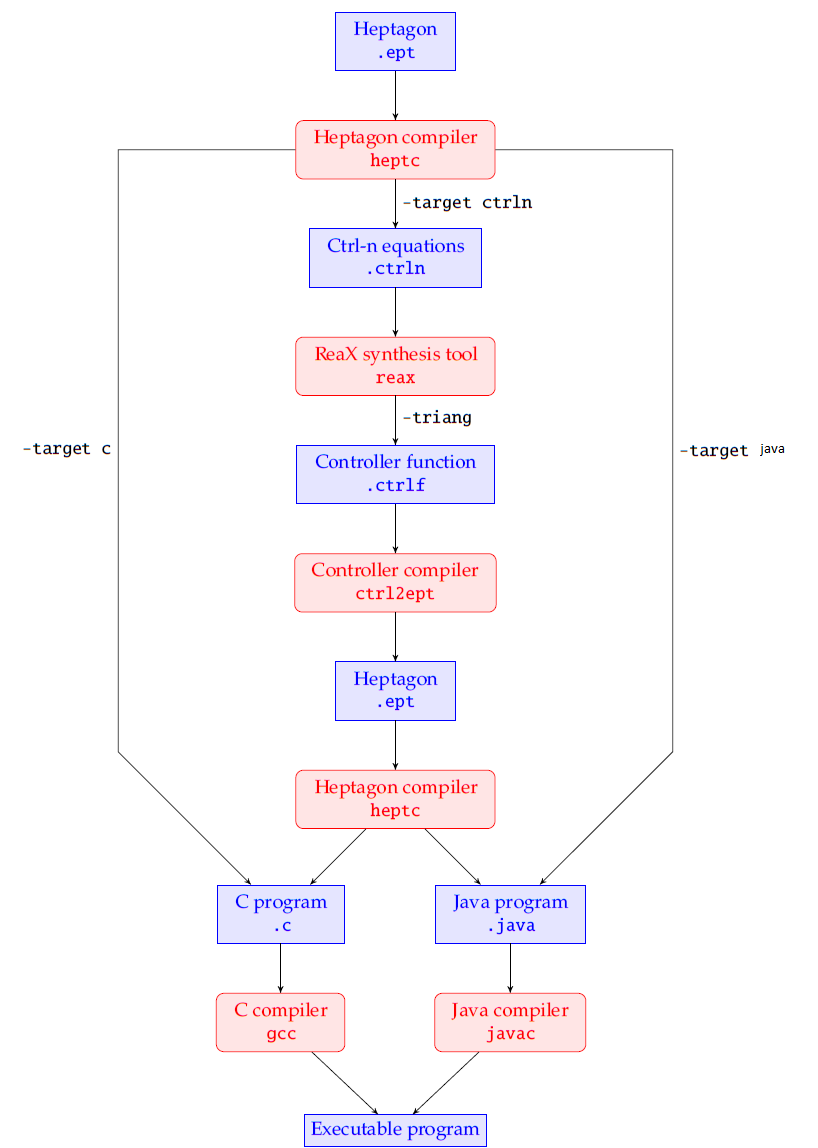
\includegraphics[height=15cm, width=15cm]{compilation.png}
 \caption{Schema de chainage de la compilation de Heptagon/BZR}
 \label{schemaCompile}
\end{figure}

\subsection*{Le code source du cas d'études}

\begin{lstlisting}
type position = Avant|Arriere|Null
type porte = Ouvert|Fermer
type lum = Rouge|Vert|Jaune
type stat = Arret|EnMouvement
node presence(presence:bool) returns (occuper:bool)
let
 automaton
  	state Nothing
 	do
    		occuper = false;
  	unless presence then Presence
  
 	state Presence
 	do
   		occuper = true;
 	unless not presence then Nothing
 end

tel

node sens(presence,entree,sortie:bool) returns (pos:position)
let
 automaton
	state NoPresence
	do
		pos = Null;
	unless entree then Avant
	|not entree & sortie then Arriere
  	state Avant
 	do
    		pos = Avant;
  	unless sortie & not entree then Arriere
	|not not presence then NoPresence
 	state Arriere
 	do
   		pos = Arriere;
 	unless entree then Avant
	|not presence then NoPresence
 end

tel

node presenceSens(entree,sortie:bool) returns (pos:position)
let
 automaton
	state Idle
	do
		pos = Null;
	unless entree then Avant
	|not entree & sortie then Arriere
  	state Avant
 	do
    		pos = Avant;
  	unless not entree & not sortie then Idle
	| sortie & not entree then Arriere
 	state Arriere
 	do
   		pos = Arriere;
 	unless entree then Avant
	|not entree & not sortie then Idle
 end

tel


node lampe(interrupteur:bool) returns (lumiere:bool)
let
 automaton
   	state Off  
	do
		lumiere = false;
	unless interrupteur then On   

	state On
	do
		lumiere = true;
	unless not interrupteur then Off
 
 end
tel

node poubelle (con,coff:bool) returns (ouvrir: bool)
let
	 automaton
		state Fermer
 		do
    			ouvrir = false;
  		unless con then Ouvrir
  
 		state Ouvrir
 		do
   			ouvrir = true;
 		unless coff then Fermer
	end
tel

node porte (copen:bool) returns (ouvrir: porte)
let
	 automaton
		state Fermer
 		do
    			ouvrir = Ouvert;
  		unless copen then Ouvrir
  
 		state Ouvrir
 		do
   			ouvrir = Fermer;
 		unless not copen then Fermer
	end
tel


node stores (copen,close: bool) returns (store: bool)
let
	 automaton
		state Fermer
 		do
    			store = false;
  		unless copen then Ouvrir
	
 		state Ouvrir
 		do
			store = true;
 		unless close then Fermer
	end
tel

node alarme (marcheArret,code,pbGar,pbHab:bool;dReprise,dVigilence,
	    dAlarme:int) returns (sonnerAlarme:bool; enMarche:lum)
var 
last temps:int = 0;
last vigilence:int = 0;
last reprise:int = 0;
let
	automaton
		state Arret
			do 
				sonnerAlarme = false;
				enMarche = Rouge;
			unless marcheArret then Allume
		state Allume
			do 
				enMarche = Vert;
				sonnerAlarme = false;
				temps = 0 fby (temps +1);
			until code then Vigilence
			| pbHab then Sonner
			| pbGar & (dVigilence <= temps) then Sonner
		state Sonner
			do 
				enMarche = Vert;
				sonnerAlarme = true;
				reprise = 0 fby (reprise +1);
			until code then Arret
			|dReprise <= reprise then Allume
		state Vigilence
			do 
				enMarche = Jaune;
				sonnerAlarme = false;
				vigilence = 0 fby (vigilence +1);
			until pbHab then Sonner
			| dVigilence <= vigilence then Arret
	end;
tel

node ascenseur(demandeEtage,arriveEtage:bool) returns (etat: bool)
let
	automaton
		state Stop
		do
			etat = false;	
		unless demandeEtage then Mouvement

		state Mouvement
		do
			etat = true;
		unless not demandeEtage or arriveEtage then Stop
	end
tel

node smartHome (presenceMaison,presenceAscenseur,presenceGarage,
		presenceDevantPoubelle,vent,luminosite,marcheArretAlarme,
		codeAlarme,codePorte,codeBarriere,presenceEntreePorte,
		presenceSortiePorte,presenceEntreeBarriere,
		presenceSortieBarriere:bool; dReprise,dVigilence,
		dAlarme:int) returns (etatMaison,lumiere,poubelleOuvert,
		ouvertureStore,alarmeSonne,property: bool;porteStatus,
	    barriere:porte;etatAlarme:lum;capteurPositionPorte,
	    capteurPositionBarriere:position;ascenseur:bool)
contract
assume true
enforce property
with (interrupteur,copen,close,openPorte,openBarriere,con,
      coff,demandeEtage,arriveEtage:bool)

var
loccuperMaison,loccuperGarage,loccuperAscenseur,lpresencePoubelle,
lLumiere,louvrirPoubelle,lstores,lsonnerAlarme,lascenseur,
prop1,prop2,prop3, prop4,prop5,prop6,prop7,prop8,prop8a,prop9,
prop10,prop11,prop12,prop13,prop14,prop15,prop16,prop12a,prop12b,
prop17,prop18,prop19,prop20, prop21,prop22,prop23,prop24,
prop25,prop26:bool;
louvrirPorte,louvrirBarriere:porte;
lenMarche:lum;
lpositionDevantPorte, lpositionDevantBarriere: position;

let
	loccuperMaison = inlined presence(presenceMaison);
	loccuperGarage = inlined presence(presenceGarage);
	loccuperAscenseur = inlined presence(presenceAscenseur);

	lLumiere = inlined lampe(interrupteur) ;
	lpresencePoubelle = inlined presence(presenceDevantPoubelle) ;
	louvrirPoubelle = inlined poubelle(con, coff);

	louvrirPorte = inlined porte (openPorte);
	lpositionDevantPorte = inlined presenceSens(presenceEntreePorte,
				presenceSortiePorte);

	louvrirBarriere = inlined porte (openBarriere);
	lpositionDevantBarriere = inlined presenceSens(presenceEntreeBarriere,
				  presenceSortieBarriere);

	lstores = inlined stores (copen,close);
	(lsonnerAlarme, lenMarche) = inlined alarme(marcheArretAlarme,
				      codeAlarme,loccuperGarage,loccuperMaison,
				      dReprise,dVigilence,dAlarme);
	lascenseur  = inlined ascenseur(demandeEtage,arriveEtage);
	
	prop1 = loccuperMaison or not lLumiere;
	prop2 = loccuperMaison or not lstores;
	prop3 = not loccuperMaison or (lstores or lLumiere);
	
	prop4 = vent or lstores;
	prop5 = not luminosite or lstores;
	prop6 = not vent or not lstores;	
	prop7 = luminosite or not lstores;
	
	prop8 = lstores or lLumiere;
	prop8a = not (not lstores & loccuperMaison) or lLumiere;
	prop9 = not lstores or not lLumiere;

	prop10 = lpresencePoubelle or not louvrirPoubelle;
	prop11 = not lpresencePoubelle or louvrirPoubelle;
	
	prop12 = not (not vent & luminosite) or lstores;
	prop12a = not (not vent & luminosite & loccuperMaison) or lstores;
	prop12b = not (not vent & luminosite & not loccuperMaison) 
		  or not lstores;
	prop13 = not (vent & not luminosite) or not lstores;
	prop14 = not (vent & luminosite) or not lstores;	
	prop15 = not (not vent & not luminosite) or not lstores;

	prop17 = not (lpositionDevantPorte = Arriere) or 
		  (louvrirPorte = Ouvert);
	prop23 = not (lpositionDevantPorte = Null) or 
		  (louvrirPorte <> Ouvert);
	prop16 = not (codePorte & lpositionDevantPorte = Avant) or 
		  (louvrirPorte = Ouvert);	

	prop19 = not (lpositionDevantBarriere= Arriere) or
		  (louvrirBarriere = Ouvert);
	prop24 = not (lpositionDevantBarriere= Null) or 
		  (louvrirBarriere <> Ouvert);
	prop18 =  not (codeBarriere & lpositionDevantBarriere = Avant) 
		  or (louvrirBarriere = Ouvert);
	
	prop20 = loccuperAscenseur or  not lascenseur;
	prop21 = not loccuperAscenseur or lascenseur;
	prop22 = loccuperMaison or (lenMarche <> Rouge);
	property = prop1 & prop2 & prop3 & prop8a & prop9 & prop10 &
		    prop11 & prop12a & prop12b & prop13 & prop14 & 
		    prop15 & prop17 & prop18 & prop19 & prop23 & prop24 & 
		    prop16 & prop20 & prop21;

	etatMaison = loccuperMaison;
	lumiere = lLumiere;
	poubelleOuvert = louvrirPoubelle;
	porteStatus = louvrirPorte;
	capteurPositionPorte = lpositionDevantPorte;
	capteurPositionBarriere = lpositionDevantBarriere;
	barriere = louvrirBarriere;
	ouvertureStore = lstores;
	etatAlarme = lenMarche;
	alarmeSonne = lsonnerAlarme;
	ascenseur = lascenseur;
	
tel
 
\end{lstlisting}

\begin{figure}[!h]
 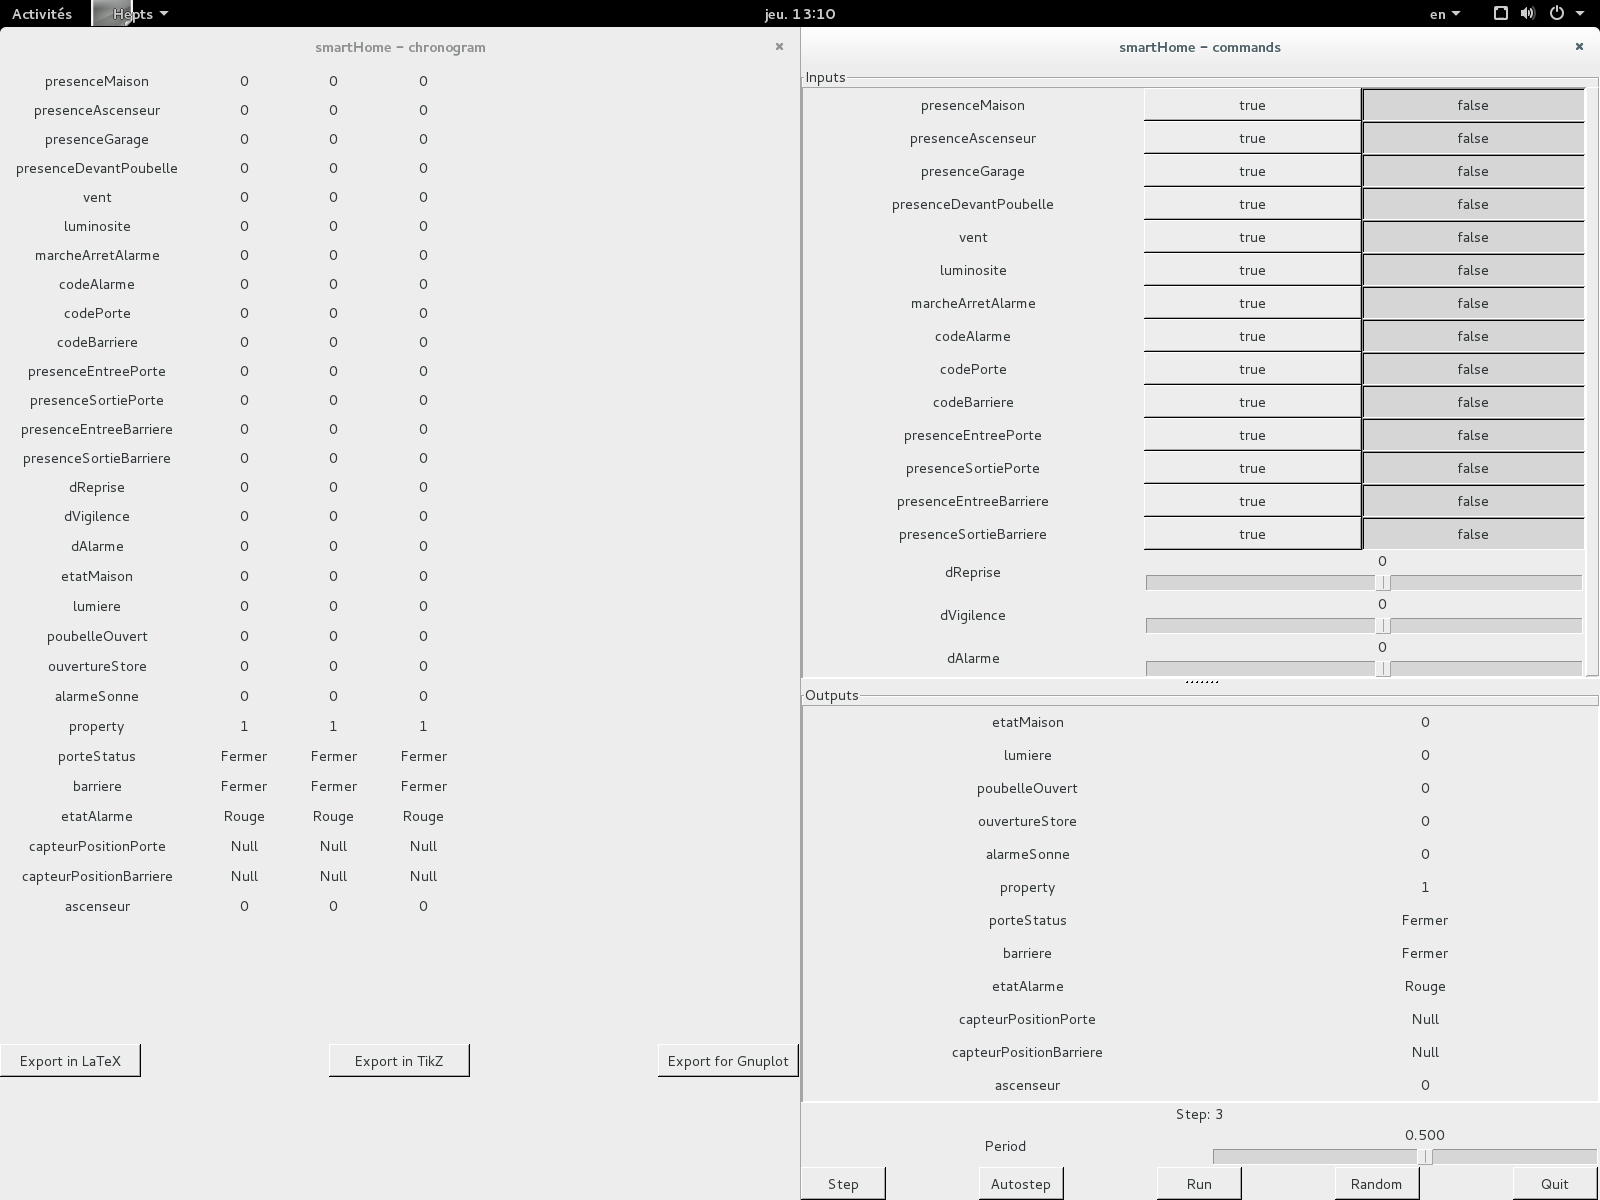
\includegraphics[height=15cm, width=15cm]{simulation.png}
 \caption{Capture de la simulation d'un exemple de modèle avec l'outil Hepts}
 \label{schemaSimilation}
\end{figure}

\subsection*{Le noeud porte}

\begin{tikzpicture}[shorten >=1pt, node distance=2cm, on grid, auto]
   \node[state, initial]            (A)                          {A};
   \node[state, accepting]          (B)   [right=of A]           {B};
   \node[state,initial,accepting]   (C)   [below right=of B]     {B'};
 
  \path[->]
             (A)  edge [bend right]   node  [swap]   {b}   (B)
                  edge [loop above]   node           {a}   ()
             (B)  edge [loop above]   node           {b}   ()
                  edge                node           {a}   (A)
                  edge [loop below]   node           {a}   ()
     
\end{tikzpicture}


\end{document}

